\begin{figure}[!h]
\centering
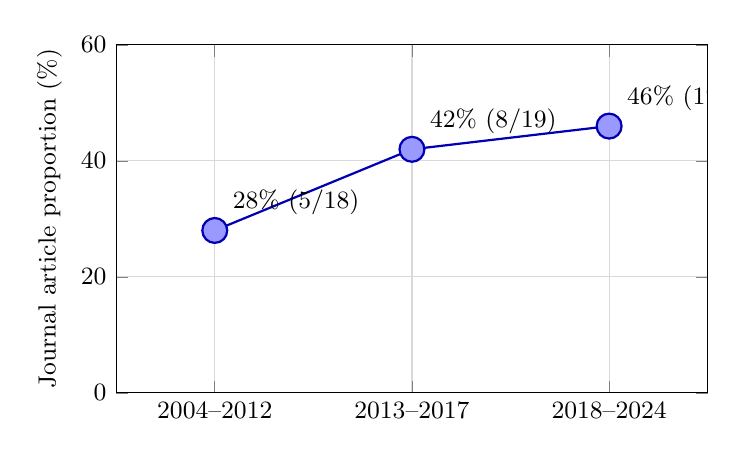
\begin{tikzpicture}
\begin{axis}[
    width=0.75\textwidth,
    height=6cm,
    ylabel={Journal article proportion (\%)},
    symbolic x coords={2004--2012, 2013--2017, 2018--2024},
    xtick=data,
    ymin=0, ymax=60,
    enlarge x limits=0.25,
    grid=major,
    grid style={gray!30},
    x tick label style={font=\small},
    y tick label style={font=\small},
    ylabel style={font=\small},
    mark size=3pt,
]

\addplot[thick, blue!70!black, mark=*, mark options={fill=blue!40, scale=1.5}]
    coordinates {
    (2004--2012, 28)
    (2013--2017, 42)
    (2018--2024, 46)
};

% Data labels with n values
\node[font=\small, anchor=south west, xshift=3pt, yshift=2pt]
    at (axis cs:2004--2012, 28) {28\% (5/18)};
\node[font=\small, anchor=south west, xshift=3pt, yshift=2pt]
    at (axis cs:2013--2017, 42) {42\% (8/19)};
\node[font=\small, anchor=south west, xshift=3pt, yshift=2pt]
    at (axis cs:2018--2024, 46) {46\% (17/37)};

\end{axis}
\end{tikzpicture}
\caption{Journal article proportion across three research periods, indicating gradual field maturation from conference-dominated to more journal-based dissemination (see Section~\ref{sec:evidence-base}).}
\label{fig:publication-type-evolution}
\end{figure}
